\documentclass{article}
\usepackage[utf8]{inputenc}
\usepackage{amsmath,amsfonts,amssymb,amsthm,mathtools}
\usepackage{parskip}
\usepackage{color}
\usepackage{booktabs}
\usepackage{tikz}
\usetikzlibrary{calc}

\newtheorem{exercise}{Exercise}
\newtheorem{answer}{Answer}

\newcommand{\dd}[2][]{\frac{\partial #1}{\partial #2}}
\newcommand{\yh}{\hat{y}}

\newcommand{\bracket}[3]{\left#1 #3 \right#2}
\newcommand{\sqb}{\bracket{[}{]}}
\renewcommand{\b}{\bracket{(}{)}}
\newcommand{\abs}{\bracket{\lvert}{\rvert}}

\newcommand{\x}{\mathbf{x}}
\newcommand{\y}{\mathbf{y}}
\newcommand{\f}{\mathbf{f}}
\newcommand{\h}{\mathbf{h}}
\renewcommand{\a}{\mathbf{a}}
\newcommand{\X}{\mathbf{X}}
\newcommand{\W}{\mathbf{W}}
\newcommand{\I}{\mathbf{I}}
\renewcommand{\P}{\operatorname{P}\b}

\newcommand{\w}{\mathbf{w}}
\newcommand{\wo}{\w^*}

\renewcommand{\L}{\mathcal{L}}
\newcommand{\E}{\operatorname{E}\sqb}
\newcommand{\Var}{\operatorname{Var}\sqb}

\newcommand{\logits}{\ell}
\newcommand{\vlogits}{\boldsymbol{\logits}}
\newcommand{\softmax}{\operatorname{softmax}\b}

\title{EMAT31530, Part 4: Neural Networks}
\author{Laurence Aitchison}
\date{}

\begin{document}

\maketitle

Most of the content this week is in the Colab notebooks.  But there's a few pages here introducing neural networks.

So far, we have worked with linear functions, of the form,
\begin{align}
  \f(\x) = \x\W.
\end{align}
And we used this function as the prediction in linear regression (with a squared error loss function), or as the logits in classification (with a maximum-likelihood objective / cross-entropy loss function).

But we can use \textit{any} function here.
So what function should we use?
Well, there's a few requirements.
\begin{itemize}
  \item lots of parameters (so gradient descent has lots of knobs to twiddle to improve the function).      
  \item doesn't reduce to something simpler.
  \item fast (e.g. uses matmuls).
\end{itemize}

We can draw the current setup as,

\begin{center}
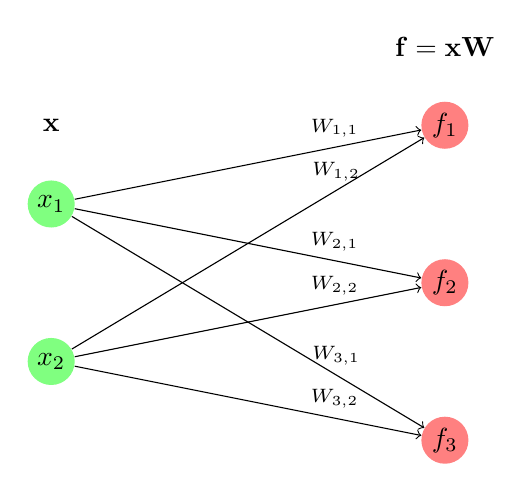
\begin{tikzpicture}
    \tikzstyle{neuron}=[circle,fill=black!25,minimum size=17pt,inner sep=0pt]
    \tikzstyle{input neuron}=[neuron, fill=green!50];
    \tikzstyle{hidden neuron}=[neuron, fill=blue!50];
    \tikzstyle{output neuron}=[neuron, fill=red!50];

    % Define the layer separation
    \def\layersep{5cm}
    \def\nodesep{2cm}

    % Draw the input layer nodes
    \foreach \name / \y in {1,2}
        \node[input neuron] (I-\name) at (0,{-(\y + 1.5)* \nodesep}) {$x_\name$};

    % Draw the output layer node
    \foreach \name / \y in {1,...,3}
        \node[output neuron] (O-\name) at (\layersep,{-(\y + 1) * \nodesep}) {$f_\name$};

    % Connect every node in the input layer with every node in the hidden layer.
    \foreach \source in {1,...,2}
        \foreach \dest in {1,...,3}
            \path[->] (I-\source) edge node[pos=0.75, above] {\scriptsize$W_{\dest, \source}$} (O-\dest) ;

    \node[above of=I-1] {$\x$};
    \node[above of=O-1] {$\f = \x \W$};


\end{tikzpicture}
\end{center}

Now, one way to get a more interesting function is to stack multiple layers (i.e. connect the outputs of one linear layer to the inputs of another layer):

\begin{center}
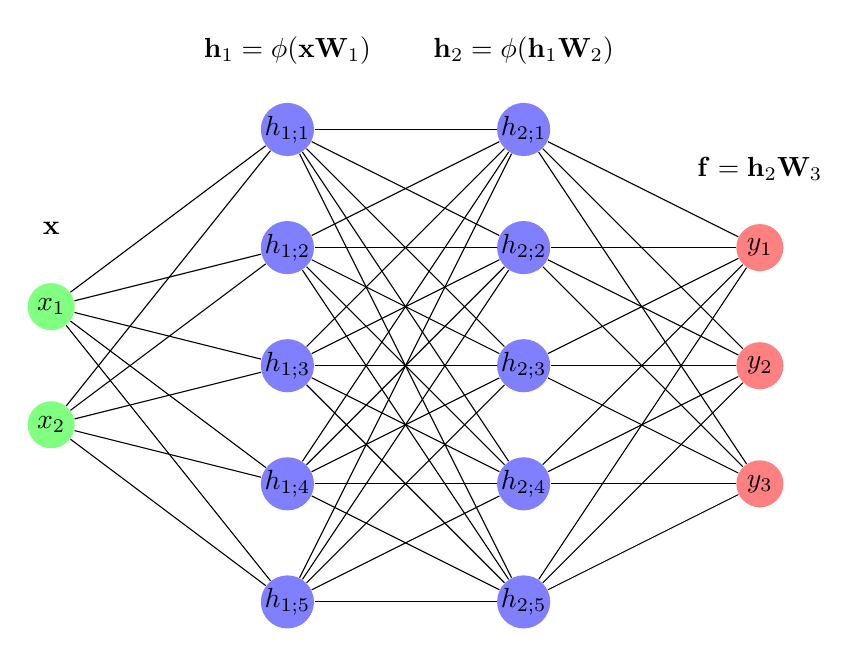
\begin{tikzpicture}
    \tikzstyle{neuron}=[circle,fill=black!25,minimum size=17pt,inner sep=0pt]
    \tikzstyle{input neuron}=[neuron, fill=green!50];
    \tikzstyle{hidden neuron}=[neuron, fill=blue!50];
    \tikzstyle{output neuron}=[neuron, fill=red!50];

    % Define the layer separation
    \def\layersep{3cm}
    \def\nodesep{1.5cm}

    % Draw the input layer nodes
    \foreach \name / \y in {1,2}
        \node[input neuron] (I-\name) at (0,{-(\y + 1.5)* \nodesep}) {$x_\name$};

    % Draw the hidden layer nodes
    \foreach \name / \y in {1,...,5}
        \node[hidden neuron] (H1-\name) at (\layersep,{-\y * \nodesep}) {$h_{1;\name}$};

    % Draw the hidden layer nodes
    \foreach \name / \y in {1,...,5}
        \node[hidden neuron] (H2-\name) at (2*\layersep,{-\y * \nodesep}) {$h_{2;\name}$};

    % Draw the output layer node
    \foreach \name / \y in {1,...,3}
        \node[output neuron] (O-\name) at (3*\layersep,{-(\y + 1)* \nodesep}) {$y_\name$};

    % Connect every node in the input layer with every node in the hidden layer.
    \foreach \source in {1,...,2}
        \foreach \dest in {1,...,5}
            \path (I-\source) edge (H1-\dest);

    \foreach \source in {1,...,5}
        \foreach \dest in {1,...,5}
            \path (H1-\source) edge (H2-\dest);

    % Connect every node in the hidden layer with the output layer
    \foreach \source in {1,...,5}
        \foreach \dest in {1,...,3}
            \path (H2-\source) edge (O-\dest);

    \node[above of=I-1] {$\x$};
    \node[above of=H1-1] {$\h_1 = \phi(\x \W_1)$};
    \node[above of=H2-1] {$\h_2 = \phi(\h_1 \W_2)$};
    \node[above of=O-1] {$\f = \h_2 \W_3$};

\end{tikzpicture}
\end{center}

Note that we have included an ``nonlinearity'', $\phi$.
This nonlinearity is necessary, because without it (or if we set $\phi(\h) = \h$), we end up with,
\begin{subequations}
\begin{align}
  \h_1 &= \x \W_1\\
  \h_2 &= \h_1 \W_2\\
  \f &= \h_2 \W_3
\end{align}
\end{subequations}
If we substitute $\h_1$ into the expression for $\h_2$, and $\h_2$ into the expression for $\f$, we end up with,
\begin{align}
  \f &= \x \underbrace{\W_1 \W_2 \W_3}_{=\W} = \x \W.
\end{align}
This is again just a linear combination of the inputs, $\x$, so offers no advantages over the original linear model.

Including a nonlinearity prevents the collapse back to a linear model, giving us a strictly more powerful class of models.
\begin{subequations}
\begin{align}
  \h_1 &= \phi(\x \W_1)\\
  \h_2 &= \phi(\h_1 \W_2)\\
  \f &= \h_2 \W_3
\end{align}
\end{subequations}
There are lots of different choices for the nonlinearity.  Perhaps the most common is the ``rectified linear unit'' or ReLU,
\begin{align}
  \phi_\text{ReLU}(a) &= \begin{cases}    
    a & \text{if } a > 0\\
    0 & \text{otherwise}
  \end{cases}  
\end{align}
This is commonly known as a 3-layer network, as there are three weight-matrices.

\begin{center}
  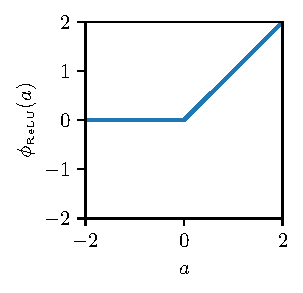
\includegraphics{relu}
\end{center}

\textbf{Q: Why don't we have a nonlinearity in the final layer (i.e.\ for producing the output, $\f$)?}
Nonlinearities can impose constraints on their outputs.
For instance, ReLU can't return negative numbers.
Alternatively, in the 1990's people sometimes used a sigmoid as a nonlinearity, but that can only output numbers between $0$ and $1$.
We don't want to impose such constraints on our outputs, which is why we don't apply the output at the final layer.

\textbf{Q: Is there a better way of understanding what nonlinearities are doing than just ``not being linear''?}
Yes ... but you need quite a bit of theory to get there.

\textbf{Q: Why is relu far more commonly used than e.g. sigmoid?}
This is to do with propagation of the gradients.
Specifically, the gradients of the sigmoid are often very small: if $h = \phi_\text{sigmoid}(a) = \sigma(a)$, 
\begin{center}
  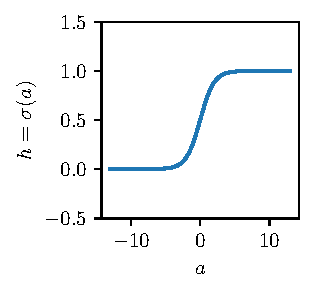
\includegraphics{sigmoid}
\end{center}
then the gradient, $\partial h / \partial a$, is small for large positive or large negative $a$.
That makes gradient descent difficult, as lots of the gradients get too small.
In contrast, the gradients for relu don't explode/vanish, as the gradient, $\partial h / \partial a = 1$ for all $a>0$.

\section{Exercises}

There are no exercises this week!  (See CoLab notebooks).


\end{document}

